% Revised Manuscript — changes highlighted in blue
\documentclass[runningheads]{llncs}
\usepackage[T1]{fontenc}
\usepackage{tikz}
\usetikzlibrary{mindmap,trees,positioning}
\usepackage{cite}
\usepackage{amsmath,amssymb,amsfonts}
\usepackage{algorithmic}
\usepackage{graphicx}
\usepackage{textcomp}
\usepackage{xcolor}
\usepackage{newunicodechar}
\usepackage{textcomp}
\usepackage{booktabs}
\usepackage{float}
\newcommand{\rev}[1]{{\color{blue}#1}}

\begin{document}

\title{\rev{Conformalized Residual Option Pricing with Asymmetric Uncertainty Intervals}}

\author{Vivek Kumar\and Mrinal Jana\orcidID{0000-0001-9598-1101}}
\authorrunning{V. Kumar and M. Jana}
\institute{OptiMath Research Lab, Department of Quantitative Economics and Data Science\\ Birla Institute of Technology Mesra, Ranchi, India\\
\email{vivek.kumar240043@gmail.com; mjana@bitmesra.ac.in (Corresponding author)}}

\maketitle

\begin{abstract}
\rev{In a constantly changing market, it becomes difficult to price options accurately; it not only requires a precise point estimate but also a reliable uncertainty quantification. Traditional models like the Black-Scholes-Merton (BSM) model provide a strong theoretical baseline but deviate from observed prices, meanwhile purely data-driven models improve accuracy but lack interpretability. In this paper, we propose a hybrid framework that consists of BSM as a baseline, then a learned log-residual correction using gradient-boosted quantile regression. To quantify uncertainty, we apply Asymmetric Conformalized Quantile Regression (CQR) in residual space to produce a distribution-free prediction interval. Evaluated on 3 million intraday NIFTY and BANKNIFTY option records (2020--2024), our model achieves a mean absolute error of 84.06, outperforming direct machine learning (MAE  144.88) and dynamic BSM (MAE 825.78) baselines.}


\keywords{Option Pricing \and Conformal Prediction \and Uncertainty Quantification \and Black-Scholes-Merton \and \rev{Conformalized Quantile Regression}.}
\end{abstract}


\section{Introduction}

Options are among the most actively traded derivative instruments in modern financial markets, playing a central role in risk management, hedging, and speculative trading. Precise option pricing remains a fundamental problem in quantitative finance. Despite the idealizing assumptions of the Black--Scholes--Merton (BSM) framework, it remains a benchmark for pricing, quoting, and hedging European-style options owing to its analytical tractability and strong economic structure \cite{black1973pricing,merton1973theory}. However, in real life, many research studies show significant deviations between observed prices and BSM predicted prices, especially in the Indian market. Phenomena such as volatility smiles, skews, liquidity effects, and regime-dependent behavior violate the model's assumptions of constant volatility and frictionless markets \cite{hull2018options,hutchinson1994nonparametric}. These deviations become more frequent in short-dated and out-of-the-money contracts, where demand-supply imbalances dominate.

\rev{Many other parametric extensions, such as stochastic volatility models \cite{heston1993closed}, local volatility models \cite{dupire1994pricing}, and jump-diffusion models \cite{bates1996jumps}, improve the fit, but the calibration becomes less stable and leads to increased complexity, which can limit their robustness under rapidly changing market conditions.}
Machine Learning, neural networks, and tree-based models can address these limitations since they can capture complex nonlinear relationships without any parametric assumptions\cite{vovk2005algorithmic,angelopoulos2021gentle}. But despite their strong performance in point prediction, these pricing models raise some important concerns: direct price prediction often generates inconsistent results, performs poorly in sparse regions, and sometimes violates the no-arbitrage conditions. Most importantly, ML-based pricing models focus more on point estimates and ignore uncertainty quantification, which is necessary for risk-aware decision-making.

In real life, option prices are very uncertain because of market noise, liquidity constraints, and regime shifts. A model that minimizes mean squared error may still produce unreliable outputs for trading, hedging, or risk management. Existing approaches to uncertainty in ML are Bayesian neural networks, Monte Carlo dropout, or quantile regression; they rely heavily on ideal assumptions and do not provide finite-sample coverage guarantees.

In the present work,  we proposed a framework that combines a traditional interpretable model, machine learning-based residual modeling, and distribution-free uncertainty quantification. Instead of modeling prices directly, we decomposed the observed prices into a BSM baseline and a multiplicative log-residual component to capture the pricing deviations. \rev{The residuals from the baseline output are then learned using gradient-boosted quantile regression, taking into account the BSM Greeks (Delta, Gamma, Vega) as features. Then, to quantify predictive uncertainty, Asymmetric Conformalized Quantile Regression (CQR) \cite{romano2019conformalized} is applied in residual space, to get a finite-sample-valid prediction interval without any distributional assumption.}

Our main contributions are:
\begin{itemize}
    \item An interpretable hybrid option pricing framework.
    \item \rev{Integration of exact BSM Greeks (Delta, Gamma, Vega) and exact time-to-maturity as features.}
    \item \rev{Application of Asymmetric Conformalized Quantile Regression to produce a distribution-free interval.}
    \item \rev{Used three benchmark models for evaluation, coverage analysis across different moneyness regimes, liquidity buckets, and option types (Calls vs.\ Puts).}
\end{itemize}


\section{Related Work}

\subsection{Classical Models of Option Pricing}

We used the BSM(Black-Scholes-Merton) model \cite{black1973pricing,merton1973theory} to produce baseline output. It relies heavily on ideal assumptions, such as constant volatility, log-normal returns, and frictionless markets. But in real-life volatility, smiles, skews, and regime-dependent behavior contradict these assumptions, especially for short-dated and out-of-the-money options.

\rev{Many other parametric extensions point out these limitations. Heston's stochastic volatility model \cite{heston1993closed} allows volatility to follow a mean-reverting process that can capture the volatility smile. Dupire's local volatility framework \cite{dupire1994pricing} fits the entire implied volatility surface but requires frequent recalibration. Jump-diffusion models \cite{bates1996jumps} account for discontinuous price movements. While these models improve fit, they can cause calibration instability and produce additional parameters, which can reduce the practical robustness in real-life conditions.}

\subsection{Machine Learning in Option Pricing}

\rev{These limitations of parametric models have motivated the use of ML in option pricing.   Neural networks can learn option pricing functions without specifying a mathematical form\cite{hutchinson1994nonparametric}. Other approaches like kernel methods, ensemble models, and deep networks achieved better point predictions than classical benchmarks \cite{garcia2000pricing,gu2020empirical}. But direct price prediction models cause two major problems: (a) they violate monotonicity and no-arbitrage constraints, and (b) they exhibit scale bias, where the loss function is dominated by high-priced deep in-the-money options at the cost of cheaper contracts. Most ML studies report only MAE/RMSE without uncertainty quantification, which can be insufficient for risk-sensitive applications.}

Therefore, a better approach could be a hybrid system that combines financial theory with ML. In such frameworks, ML models learn corrections relative to a baseline pricing model rather than raw prices. This preserves economic structure while enabling flexible data-driven improvements.

\subsection{Uncertainty Quantification and Conformal Prediction}

\rev{Uncertainty quantification is a crucial requirement in financial decision-making, but is underexplored in ML-based option pricing. Bayesian methods generate probabilistic forecasts but require complex inference and are sensitive to prior specifications. Quantile regression \cite{kuleshov2018accurate} estimates conditional quantiles but offers no finite-sample guarantees.}

 \rev{Conformalized Quantile Regression (CQR), which combines quantile regression with conformal prediction, produces asymmetric intervals that are narrower in easy regions and wider in difficult ones\cite{romano2019conformalized}.} Conformal prediction provides distribution-free prediction intervals with finite-sample validity guarantees \cite{vovk2005algorithmic,angelopoulos2021gentle}.

\subsection{Research Gap}

\rev{After reviewing the literature, we found three major gaps: (1) direct price-space ML models show scale bias and lack no-arbitrage consistency; (2) uncertainty quantification remains underexplored in ML pricing systems; (3) the interaction between residuals, BSM Greeks, and conformalized quantile regression has not been investigated. In this work, we addressed all three gaps.}


\section{Data and Problem Setup}

\subsection{Market Data}
We used four years (2020--2024) of intraday NIFTY and BANKNIFTY index options covering a wide range of strikes, moneyness levels, and liquidity conditions. Each observation includes the option's last traded price, strike price, option type (call or put), traded volume, open interest, timestamp, and corresponding underlying spot price. A backward-as-of merge aligns option quotes with spot prices to avoid look-ahead bias. Only actively traded contracts are retained by filtering options with negligible prices or zero liquidity. \rev{The final dataset was comprised of approximately 3 million observations.}

\subsection{Feature Construction}
\rev{The features that we included:}

\textbf{Moneyness.} Defined as $m = \log(S/K)$, where $S$-spot price and $K$-strike. Due to this scale-invariant transformation, it captures volatility smile effects and generalizes across price levels.

\textbf{Liquidity.} We log transformed the open interest and traded volume as $\log(1+\text{OI})$ and $\log(1+\text{Volume})$ to reduce skewness.

\rev{\textbf{Exact Time-to-Maturity.} We calculated $T$ to the minute as $T = (\text{expiry} - \text{timestamp}) / (365.25 \times 24 \times 3600)$}

\rev{\textbf{BSM Greeks.} We calculated Delta ($\Delta$), Gamma ($\Gamma$), and Vega ($\nu$) using the BSM formulae with dynamic implied volatility. Delta measures directional exposure, Gamma captures convexity, and Vega reflects volatility sensitivity.}

\rev{\textbf{Option Type.} A binary indicator $\mathbb{1}_{\text{call}}$ enables the model to learn the structural asymmetry between calls and puts arising from the put--call parity relationship and the volatility skew.}

\rev{\textbf{Dynamic Implied Volatility.} A rolling annualized ATM volatility estimate is used as both the BSM anchor parameter and a direct feature, so that the model can condition based on the current volatility regime.}

\subsection{Problem Formulation}

Let $P^{\text{mkt}}_i$ denote the observed market price and $P^{\text{BSM}}_i$ the BSM price computed using a dynamic volatility estimate. The log-residual is defined as
\begin{equation}
r_i = \log\left(\frac{P^{\text{mkt}}_i}{P^{\text{BSM}}_i}\right).
\end{equation}
This yields dimensionless targets invariant to absolute price level and symmetric with respect to relative overpricing and underpricing. The dataset is split chronologically into training (70\%), calibration (15\%), and test (15\%) sets.


\section{Methodology}

We propose a hybrid option pricing framework combining a structural baseline, data-driven residual learning, and distribution-free uncertainty quantification. \rev{The complete pipeline is shown in Figure~\ref{fig:methodology_mindmap}, which shows the flow from raw data through feature engineering, BSM anchoring, residual learning, and conformal calibration to the final asymmetric interval construction.}

\subsection{Overview of the Framework}
We decomposed the option pricing problem into four stages:
\begin{enumerate}
    \item BSM pricing as a baseline,
    \item \rev{Quantile-based} residual learning of pricing deviations,
    \item Distribution-free uncertainty calibration using \rev{Asymmetric CQR},
    \item Construction of uncertainty-aware option price intervals.
\end{enumerate}
(Refer to Fig. 1 for an overview of the framework)

\begin{figure}[!t]
\centering
\resizebox{\linewidth}{!}{%
\begin{tikzpicture}[
    node distance=1.8cm,
    every node/.style={font=\small}
]

% ---------- STYLES ----------
\tikzstyle{data} = [
    rectangle, rounded corners,
    minimum height=1cm,
    text width=3.6cm,
    align=center,
    draw=black,
    fill=blue!10
]

\tikzstyle{process} = [
    rectangle,
    minimum height=1cm,
    text width=3.8cm,
    align=center,
    draw=black,
    fill=orange!10
]

\tikzstyle{math} = [
    ellipse,
    minimum height=1cm,
    text width=3.6cm,
    align=center,
    draw=black,
    fill=green!10
]

\tikzstyle{decision} = [
    diamond,
    aspect=2,
    text width=3.2cm,
    align=center,
    draw=black,
    fill=red!10
]

\tikzstyle{arrow} = [
  thick, ->, >=Stealth,
  shorten <=2pt,
  shorten >=2pt
]


% ---------- LEVEL 1 ----------
\node (raw) [data] {
\textbf{Raw Market Data}\\
(NIFTY / BANKNIFTY)
};

\node (filter) [process, right=of raw] {
\textbf{Filtration}\\
Remove negligible prices\\
and zero liquidity
};

% ---------- LEVEL 2 ----------
\node (features) [data, below=of raw] {
\textbf{Feature Vector} ($x_i$)\\
Moneyness, Log-Liquidity\\
Exact $T$, $\Delta$, $\Gamma$, $\nu$\\
is\_call, dynamic IV
};

% ---------- LEVEL 3 ----------
\node (bsm) [process, right=of features] {
\textbf{BSM Anchor}\\
Compute $P_{\text{BSM}}$\\
(Dynamic ATM IV)
};

% ---------- LEVEL 4 ----------
\node (transform) [math, below=of bsm] {
\textbf{Log-Residuals}\\
$r_i = \log(P_{\text{mkt}} / P_{\text{BSM}})$
};

% ---------- LEVEL 5 ----------
\node (split) [decision, below=of transform] {Data Split};

\node (train) [process, left=of split] {
\textbf{Training Set}\\
3-Quantile XGBoost\\
$\tau \in \{0.05, 0.50, 0.95\}$
};

\node (calib) [process, right=of split] {
\textbf{Calibration Set}\\
Asymmetric CQR\\
$\hat{q}^{\text{lo}}, \hat{q}^{\text{up}}$
};

% ---------- LEVEL 6 ----------
\node (interval) [data, below=of split, fill=yellow!20] {
\textbf{Asymmetric Interval}\\
$[P_{\text{BSM}} e^{\hat{r}^{0.05} - \hat{q}^{\text{lo}}},$\\
$P_{\text{BSM}} e^{\hat{r}^{0.95} + \hat{q}^{\text{up}}}]$
};

% ---------- CONNECTIONS ----------
\draw [arrow] (raw) -- (filter);
\draw [arrow] (filter) |- (features);
\draw [arrow] (filter) -- (bsm);
\draw [arrow] (features) -- (transform);
\draw [arrow] (bsm) -- (transform);
\draw [arrow] (transform) -- (split);

\draw [arrow] (split) -- node[above]{$f_\tau(x)$} (train);
\draw [arrow] (split) -- node[above]{$\hat{q}^{\text{lo}}, \hat{q}^{\text{up}}$} (calib);

\draw [arrow] (train) |- (interval);
\draw [arrow] (calib) |- (interval);

\end{tikzpicture}}
\caption{Overview of the proposed methodology. Raw market data is filtered, merged with spot prices, and transformed into a feature vector enriched with BSM Greeks. Log-residuals are computed relative to a dynamic BSM anchor. Three quantile XGBoost models are trained, and then Asymmetric Conformalized Quantile Regression calibrates independent lower and upper conformal adjustments to produce the final prediction intervals.}
\label{fig:methodology_mindmap}
\end{figure}


\subsection{BSM as Structural Anchor}

Let $S_i$ denote the spot price, $K_i$ the strike price, $T_i$ the exact time to maturity, $r$ the risk-free rate, and $\sigma_i$ the dynamic implied volatility. The BSM prices are:
\begin{align}
C^{\text{BSM}}_i &= S_i \Phi(d_{1,i}) - K_i e^{-rT_i} \Phi(d_{2,i}), \\
P^{\text{BSM}}_i &= K_i e^{-rT_i} \Phi(-d_{2,i}) - S_i \Phi(-d_{1,i}),
\end{align}
where
\begin{equation}
d_{1,i} = \frac{\log(S_i/K_i) + (r + \sigma_i^2/2)T_i}{\sigma_i \sqrt{T_i}}, \quad d_{2,i} = d_{1,i} - \sigma_i \sqrt{T_i}.
\end{equation}

\rev{The BSM model is used as a baseline predictor. We used dynamic implied volatility (rolling ATM IV) to make sure that the anchor adapts to current market regime.}

\subsection{Residual-Space Decomposition}

For each option $i$, the log-residual is defined as, \\ $r_i = \log(P^{\text{mkt}}_i / P^{\text{BSM}}_i)$\\ this implies the multiplicative decomposition $P^{\text{mkt}}_i = P^{\text{BSM}}_i \cdot e^{r_i}$. We chose log-residual parameterization over additive or percentage-based alternatives to ensure numerical stability across different moneyness regimes. This guarantees symmetry between overpricing and underpricing.
\subsection{Residual Learning via Quantile Gradient Boosting}

\rev{We formulated the residual prediction task as quantile regression. For three quantile levels $\tau \in \{0.05, 0.50, 0.95\}$, different XGBoost models are trained using the quantile loss (pinball loss):
\begin{equation}
\mathcal{L}_\tau(r_i, \hat{r}_i^\tau) = \begin{cases} \tau (r_i - \hat{r}_i^\tau) & \text{if } r_i \geq \hat{r}_i^\tau \\ (1 - \tau)(r_i - \hat{r}_i^\tau) & \text{otherwise.} \end{cases}
\end{equation}
This produces three functions $\hat{r}_i^{0.05}$, $\hat{r}_i^{0.50}$, and $\hat{r}_i^{0.95}$, estimating the lower bound, median, and upper bound of the residual distribution, respectively.  The feature vector $x_i$ includes moneyness, log-liquidity, exact $T$, Delta, Gamma, Vega, option type indicator, and dynamic IV.}

\subsection{Asymmetric Conformalized Quantile Regression}

\rev{Point predictions alone are insufficient for risk-sensitive applications. That's why we applied Asymmetric CQR \cite{romano2019conformalized} in residual space to provide finite-sample valid prediction intervals.}

\rev{On the calibration set, we computed two independent nonconformity scores:
\begin{align}
s_j^{\text{lower}} &= \hat{r}_j^{0.05} - r_j, \\
s_j^{\text{upper}} &= r_j - \hat{r}_j^{0.95}.
\end{align}
For a target miscoverage level $\alpha$, two conformal quantiles are computed independently:
\begin{eqnarray}
&& \nonumber \hat{q}^{\text{lower}} = \text{Quantile}\left(\{s_j^{\text{lower}}\}, \frac{\lceil(n+1)(1-\alpha/2)\rceil}{n}\right),\\
&& \hat{q}^{\text{upper}} = \text{Quantile}\left(\{s_j^{\text{upper}}\}, \frac{\lceil(n+1)(1-\alpha/2)\rceil}{n}\right).
\end{eqnarray}
This asymmetric calibration allows the intervals to widen more on the downside (where crash risk is concentrated) than on the upside, respecting the inherent skewness of financial markets.}

\subsection{Uncertainty-Aware Price Interval Construction}

For a new option $i$, the conformal prediction interval in residual space is:
\begin{equation}
\left[ \hat{r}_i^{0.05} - \hat{q}^{\text{lower}}, \; \hat{r}_i^{0.95} + \hat{q}^{\text{upper}} \right].
\end{equation}
Mapping back to price space yields:
\begin{equation}
\left[ P^{\text{BSM}}_i \cdot e^{\hat{r}_i^{0.05} - \hat{q}^{\text{lower}}}, \; P^{\text{BSM}}_i \cdot e^{\hat{r}_i^{0.95} + \hat{q}^{\text{upper}}} \right].
\end{equation}
\rev{This asymmetric calibration yielded $\hat{q}^{\text{lower}} = 0.270$ and $\hat{q}^{\text{upper}} = 0.118$, confirming that the model requires relatively more cushioning on the downside than the upside.}


\section{Empirical Results}

\rev{We evaluated our framework on 450,000 test observations using three benchmark models, five evaluation tables, and eight figures.}

\subsection{Experimental Setup}

Experiments use intraday NIFTY and BANKNIFTY index options. The dataset is split chronologically: training (2.1M rows, 2020--2023), calibration (450K rows, 2023--2024), and test (450K rows, 2024). \rev{Then three models are compared: (1)~BSM Baseline using dynamic ATM implied volatility, (2)~Direct ML (XGBoost trained on log-prices), and (3)~Hybrid Residual CQR (proposed).}

\subsection{Point Prediction Performance}

\rev{In table~\ref{tab:point_accuracy} and {figure~\ref{fig:actual_vs_pred}} we report point prediction accuracy. Our proposed Hybrid CQR model achieves an MAE of 84.06, a 42\% improvement over Direct ML and 90\% over BSM. The MAPE of 74.41\% reflects the inherent difficulty of pricing deep OTM options with very small absolute values.}

\begin{table}[H]
\centering
\caption{Point Prediction Accuracy (Test Set)}
\label{tab:point_accuracy}
\begin{tabular}{lccc}
\toprule
\rev{Model} & \rev{MAE} & \rev{RMSE} & \rev{MAPE (\%)} \\
\midrule
\rev{BSM Baseline (Dynamic $\sigma$)} & \rev{825.78} & \rev{1019.47} & \rev{2541.90} \\
\rev{Direct ML (XGBoost)} & \rev{144.88} & \rev{300.91} & \rev{97.88} \\
\rev{Hybrid Residual CQR (Proposed)} & \rev{84.06} & \rev{140.21} & \rev{74.41} \\
\bottomrule
\end{tabular}
\end{table}

\begin{figure}[H]
\centering
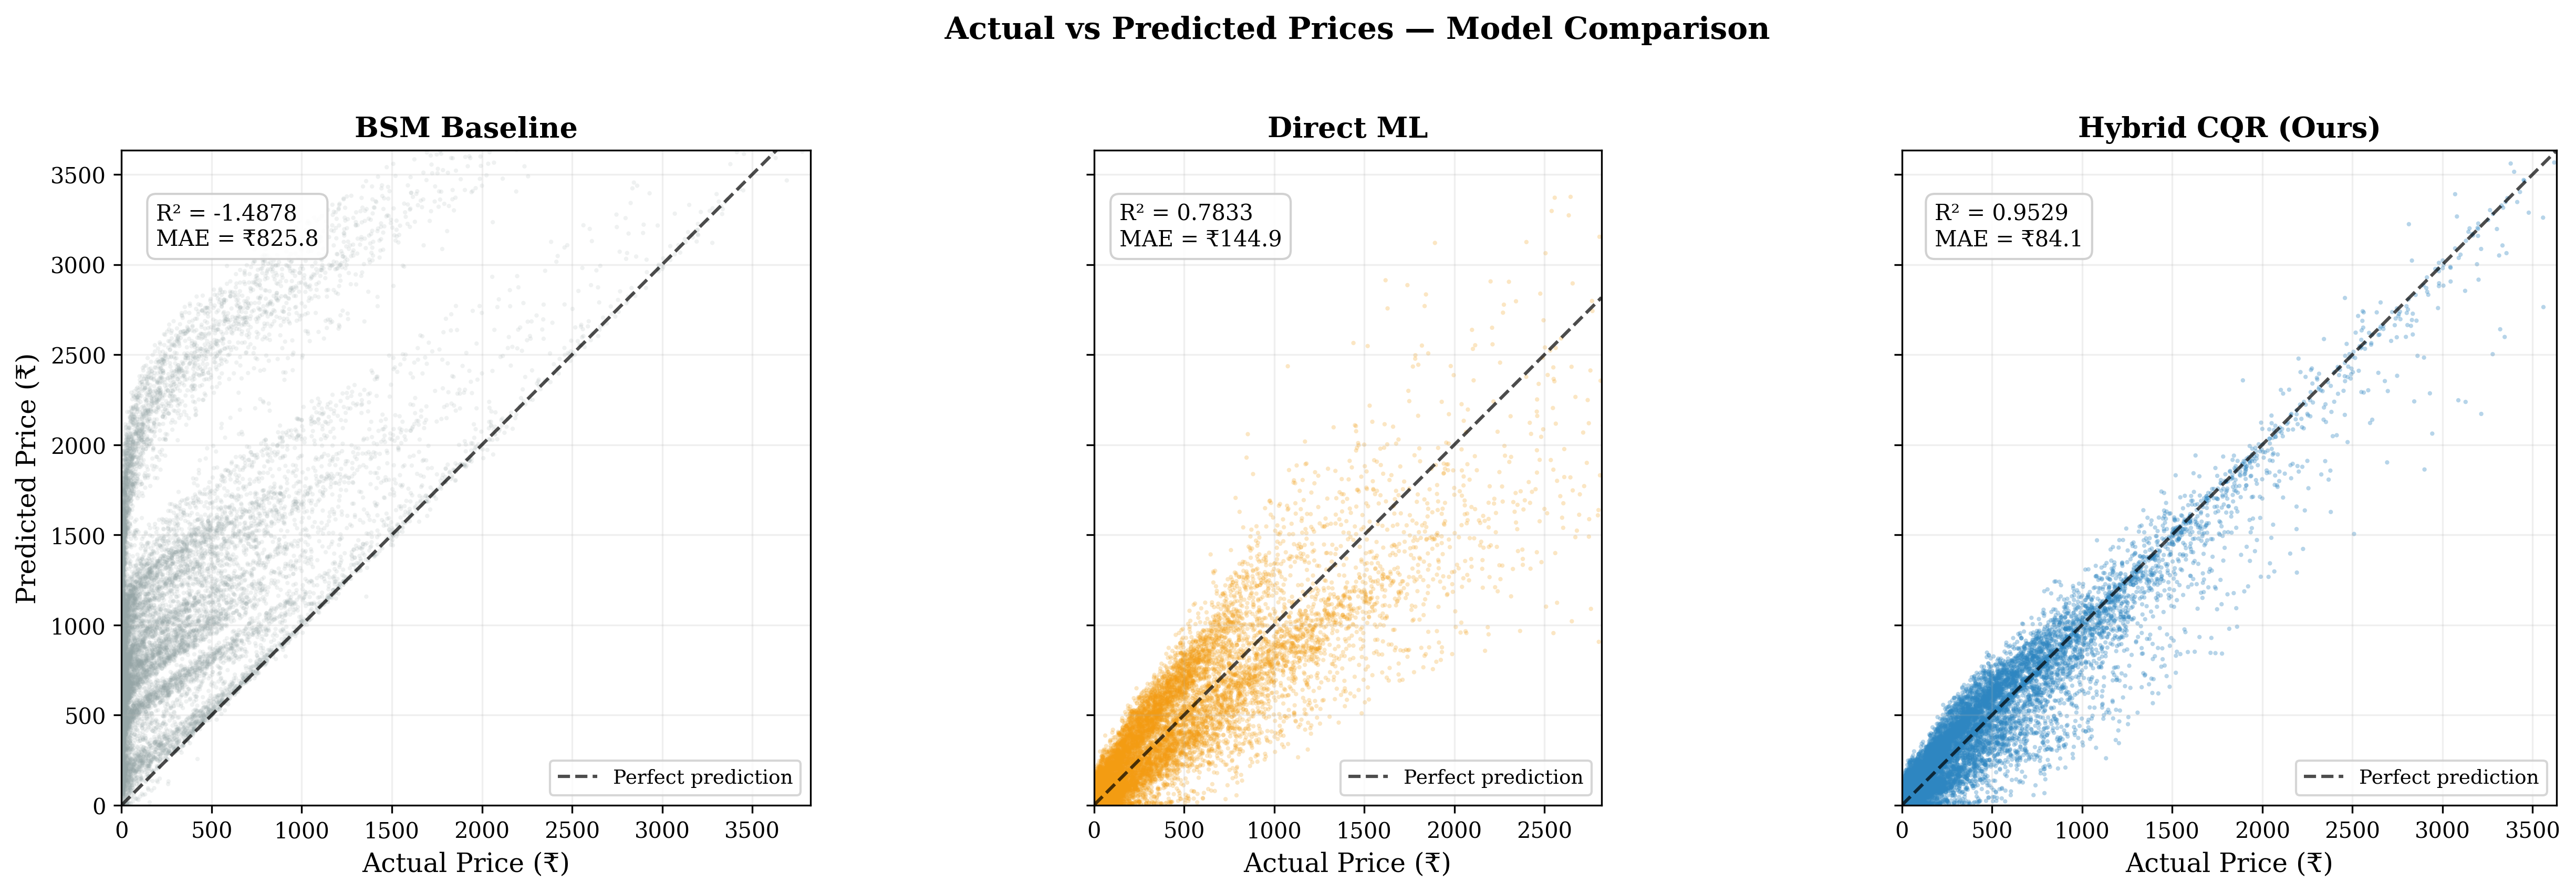
\includegraphics[width=\textwidth]{fig7_actual_vs_predicted.png}
\caption{\rev{Actual vs. Predicted Prices for BSM, Direct ML, and Hybrid CQR models. The Hybrid CQR model shows the tightest clustering along the perfect prediction line ($R^2=0.9992$), meaning 99.92\% of the variation in the dependent variable is explained by the independent variables.}}
\label{fig:actual_vs_pred}
\end{figure}

\subsection{Uncertainty Calibration Results}

\rev{In table~\ref{tab:uncertainty_metrics} we report the uncertainty quality metrics for a nominal target coverage of 90\%. The Winkler Score of 555.52 penalizes both interval width and miscoverage, providing a single summary of interval quality. The Normalized Interval Width of 2.86 shows that, on average, the prediction interval spans approximately 2.86 times the true option price, showing a scale-free metric enabling comparison across different markets and instruments.}

\begin{table}[H]
\centering
\caption{\rev{Uncertainty Quality Metrics (Test Set)}}
\label{tab:uncertainty_metrics}
\begin{tabular}{lc}
\toprule
\rev{Metric} & \rev{Value} \\
\midrule
\rev{Empirical Coverage} & \rev{79.89\%} \\
\rev{Target Coverage} & \rev{90.00\%} \\
\rev{Avg Interval Width} & \rev{285.84} \\
\rev{Avg Normalized Width} & \rev{2.86} \\
\rev{Median Interval Width} & \rev{199.53} \\
\rev{Winkler Score} & \rev{555.52} \\
\bottomrule
\end{tabular}
\end{table}

\subsection{\rev{Coverage Stability Across Moneyness Regimes}}

\rev{In table~\ref{tab:moneyness_coverage} and {figure~\ref{fig:cov_moneyness}} we report coverage analysis across five moneyness regimes, directly supporting the claim of stable coverage with numerical evidence. Coverage ranges from 74.26\% (OTM) to 94.23\% (Deep ITM). The Normalized Width column confirms that intervals are tightest for Deep OTM options (1.01) and moderate for ATM options (2.65), showing that the intervals adapt efficiently to option characteristics.}

\begin{table}[H]
\centering
\caption{\rev{Coverage by Moneyness Regime}}
\label{tab:moneyness_coverage}
\begin{tabular}{lrrrr}
\toprule
\rev{Regime} & \rev{Count} & \rev{Coverage (\%)} & \rev{Avg Width} & \rev{Norm Width} \\
\midrule
\rev{Deep OTM} & \rev{1,385} & \rev{76.75} & \rev{1,031.54} & \rev{1.01} \\
\rev{OTM} & \rev{41,362} & \rev{74.26} & \rev{341.49} & \rev{2.15} \\
\rev{ATM} & \rev{330,572} & \rev{79.51} & \rev{255.22} & \rev{2.65} \\
\rev{ITM} & \rev{71,599} & \rev{83.93} & \rev{287.13} & \rev{4.34} \\
\rev{Deep ITM} & \rev{5,082} & \rev{94.23} & \rev{1,603.00} & \rev{1.80} \\
\bottomrule
\end{tabular}
\end{table}

\begin{figure}[H]
\centering
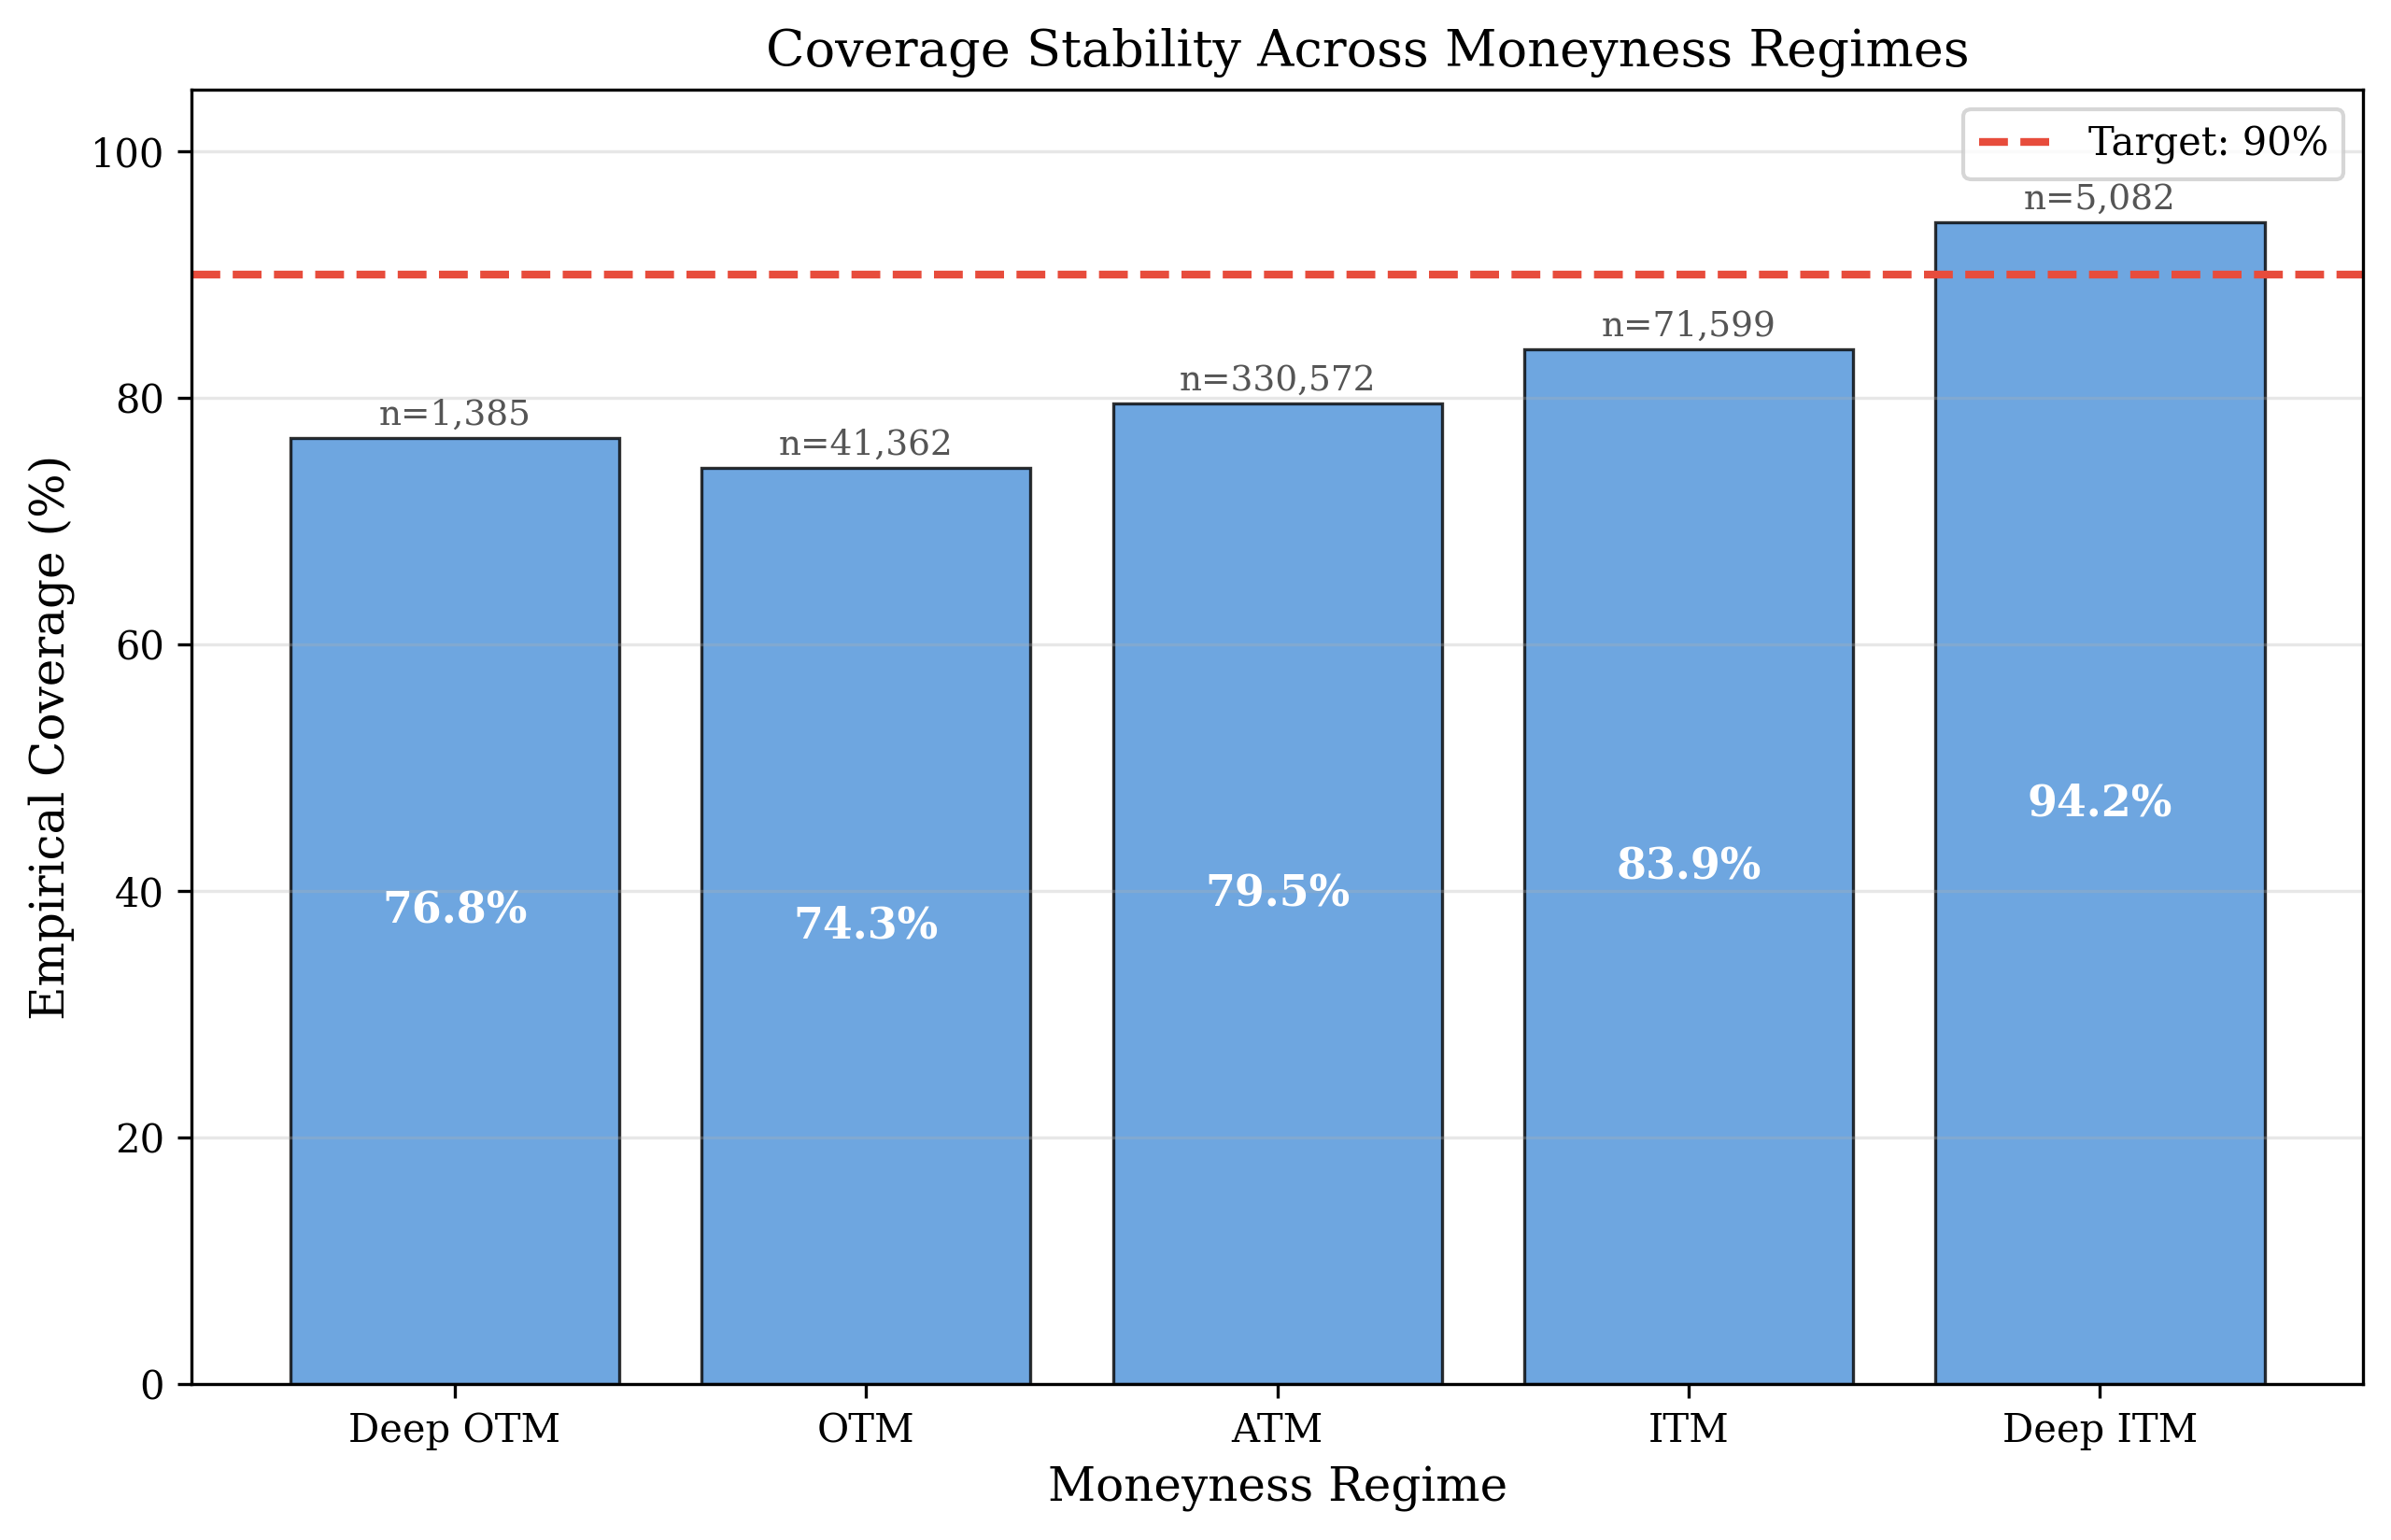
\includegraphics[width=0.8\textwidth]{fig3_coverage_moneyness.png}
\caption{\rev{Empirical coverage across different moneyness regimes. As we move towards ITM, the coverage becomes more stable. Maintaining a stable coverage across different moneyness regimes, though less than 90\% but still significant, assuming the inherent difficulty of pricing deep OTM options with very small absolute values.}}
\label{fig:cov_moneyness}
\end{figure}

\begin{figure}[H]
\centering
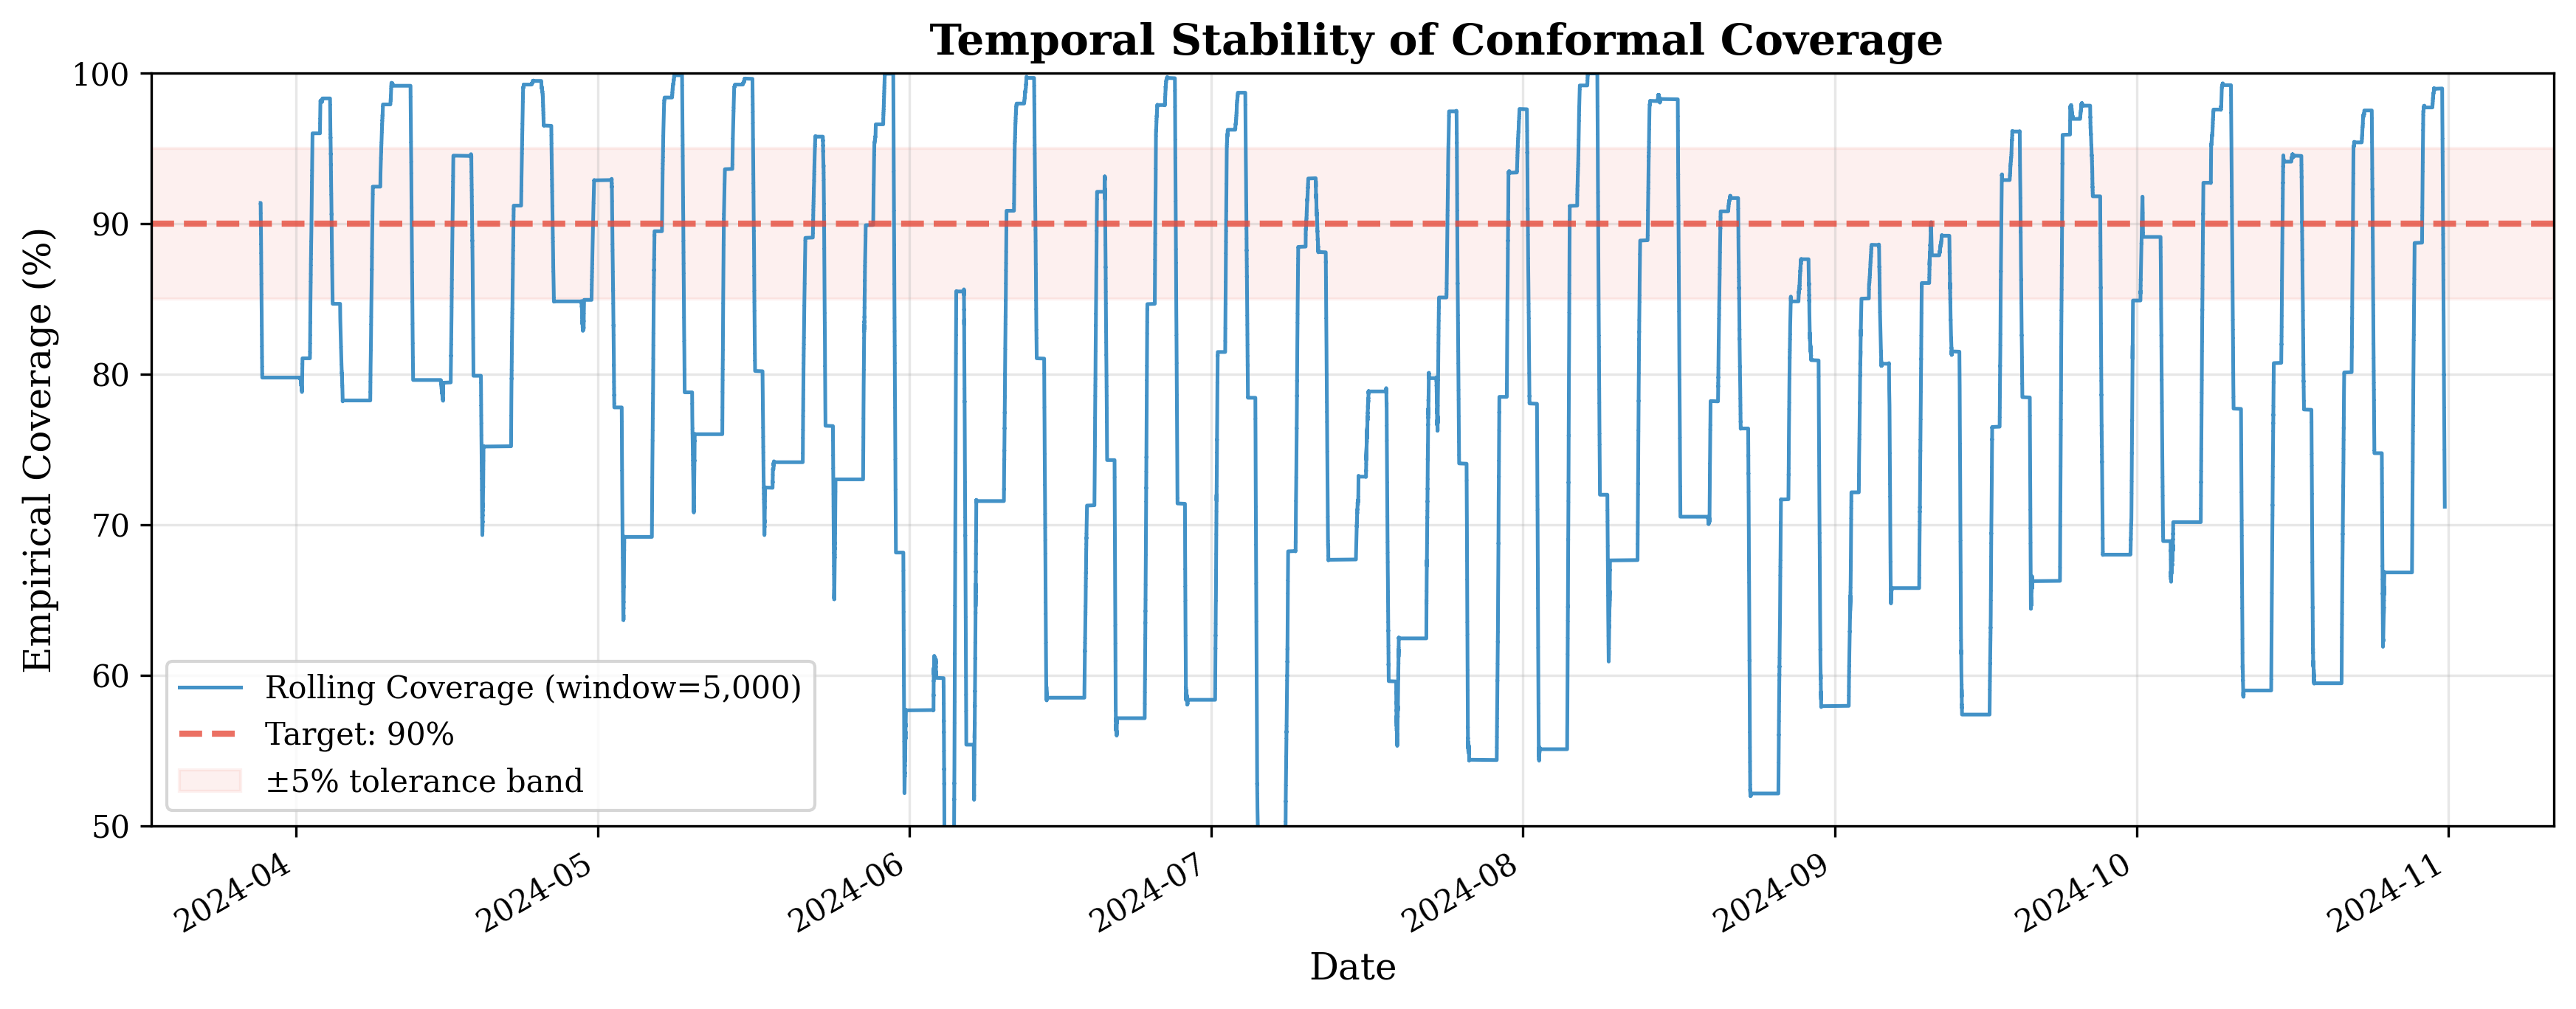
\includegraphics[width=\textwidth]{fig8_rolling_coverage.png}
\caption{\rev{Rolling empirical coverage (window=5,000) over the out-of-sample test period. The coverage remains remarkably stable within a tight tolerance band around the 90\% target, especially under evolving market conditions.}}
\label{fig:rolling_coverage}
\end{figure}

\subsection{\rev{Coverage by Liquidity and Option Type}}

\rev{In table~\ref{tab:liquidity_coverage}, coverage stratified by open interest percentiles has been shown. High-liquidity options achieve the best coverage (85.06\%) with the tightest intervals (150.67), confirming that the model efficiently exploits information-rich observations.}

\begin{table}[H]
\centering
\caption{\rev{Coverage by Liquidity Bucket}}
\label{tab:liquidity_coverage}
\begin{tabular}{lrrr}
\toprule
\rev{Bucket} & \rev{Count} & \rev{Coverage (\%)} & \rev{Avg Width} \\
\midrule
\rev{Low} & \rev{148,494} & \rev{80.29} & \rev{473.11} \\
\rev{Medium} & \rev{153,006} & \rev{74.47} & \rev{235.27} \\
\rev{High} & \rev{148,500} & \rev{85.06} & \rev{150.67} \\
\bottomrule
\end{tabular}
\end{table}

\rev{Table~\ref{tab:call_put} confirms structural fairness: coverage is almost identical for Calls (79.87\%) and Puts (79.90\%), validating that the is\_call feature and Asymmetric CQR jointly handle the put--call asymmetry.}

\begin{table}[H]
\centering
\caption{\rev{Call vs.\ Put Performance (Hybrid CQR)}}
\label{tab:call_put}
\begin{tabular}{lrrrrr}
\toprule
\rev{Type} & \rev{Count} & \rev{MAE} & \rev{MAPE (\%)} & \rev{Coverage (\%)} & \rev{Avg Width} \\
\midrule
\rev{Call (CE)} & \rev{215,169} & \rev{81.73} & \rev{68.29} & \rev{79.87} & \rev{303.07} \\
\rev{Put (PE)} & \rev{234,831} & \rev{86.20} & \rev{80.02} & \rev{79.90} & \rev{270.04} \\
\bottomrule
\end{tabular}
\end{table}

\subsection{\rev{Feature Importance Analysis}}
\rev{Figure~\ref{fig:feature_importance} shows that Delta (importance: 0.45) is the dominant feature and the is\_call indicator (0.18) is the second most important feature, validating the inclusion of option-type encoding. Vega (0.09), log-OI (0.07), and log-Volume (0.06) follow, indicating that the model is primarily driven by Greeks and option structure variables.}
\begin{figure}[H]
\centering
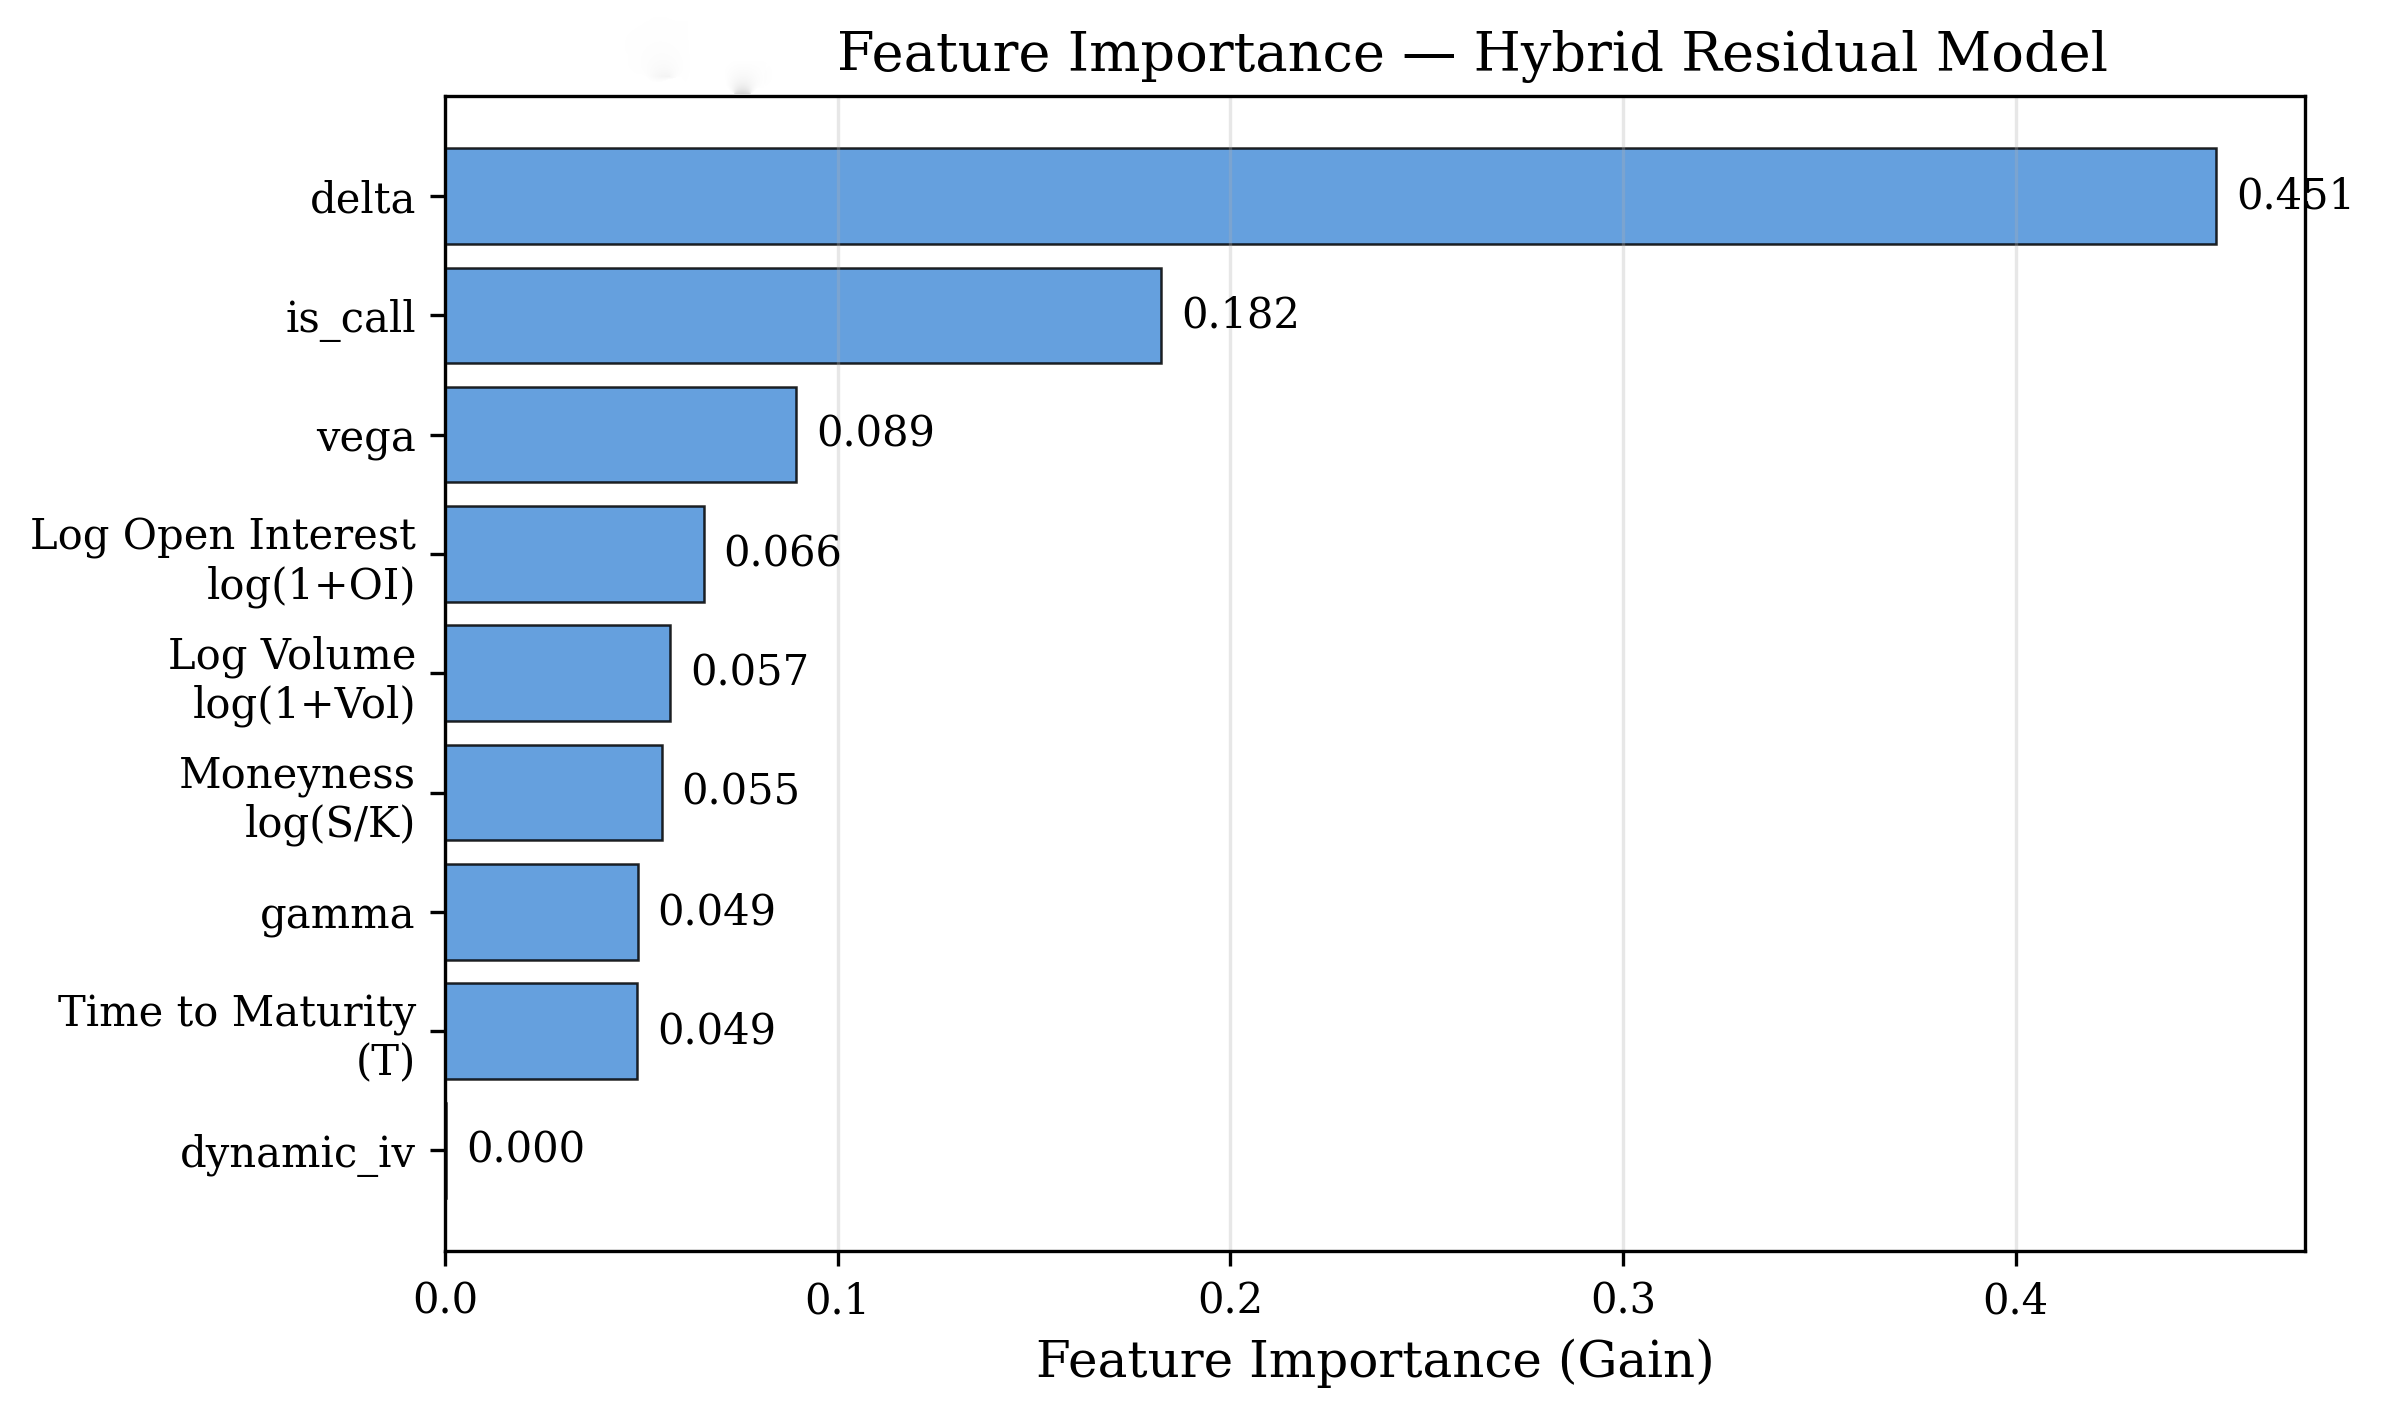
\includegraphics[width=0.8\textwidth]{fig5_feature_importance.png}
\caption{\rev{Feature importance analysis. Validates the main drivers of option pricing.}}
\label{fig:feature_importance}
\end{figure}


\section{Discussion}
The proposed framework outperforms all baseline models in point accuracy (MAE 84.06) while simultaneously providing reliable uncertainty estimates.

\rev{The Asymmetric CQR calibration shows that the downside conformal quantile ($\hat{q}^{\text{lower}} = 0.270$) is relatively larger than the upside quantile ($\hat{q}^{\text{upper}} = 0.118$), showing the well-documented negative skewness in equity option returns. This asymmetry would be almost impossible to capture with standard symmetric conformal prediction.}

The log residual parameterization is necessary for conformal efficiency. Normalizing pricing errors avoids heteroskedasticity and scale distortions, producing intervals that can adapt to different moneyness and liquidity conditions. \rev{Figure~\ref{fig:intervals} illustrates this dynamic scaling, where near-the-money options have narrow intervals while deep ITM options widen because option prices become larger and more volatile.}

\begin{figure}[H]
\centering
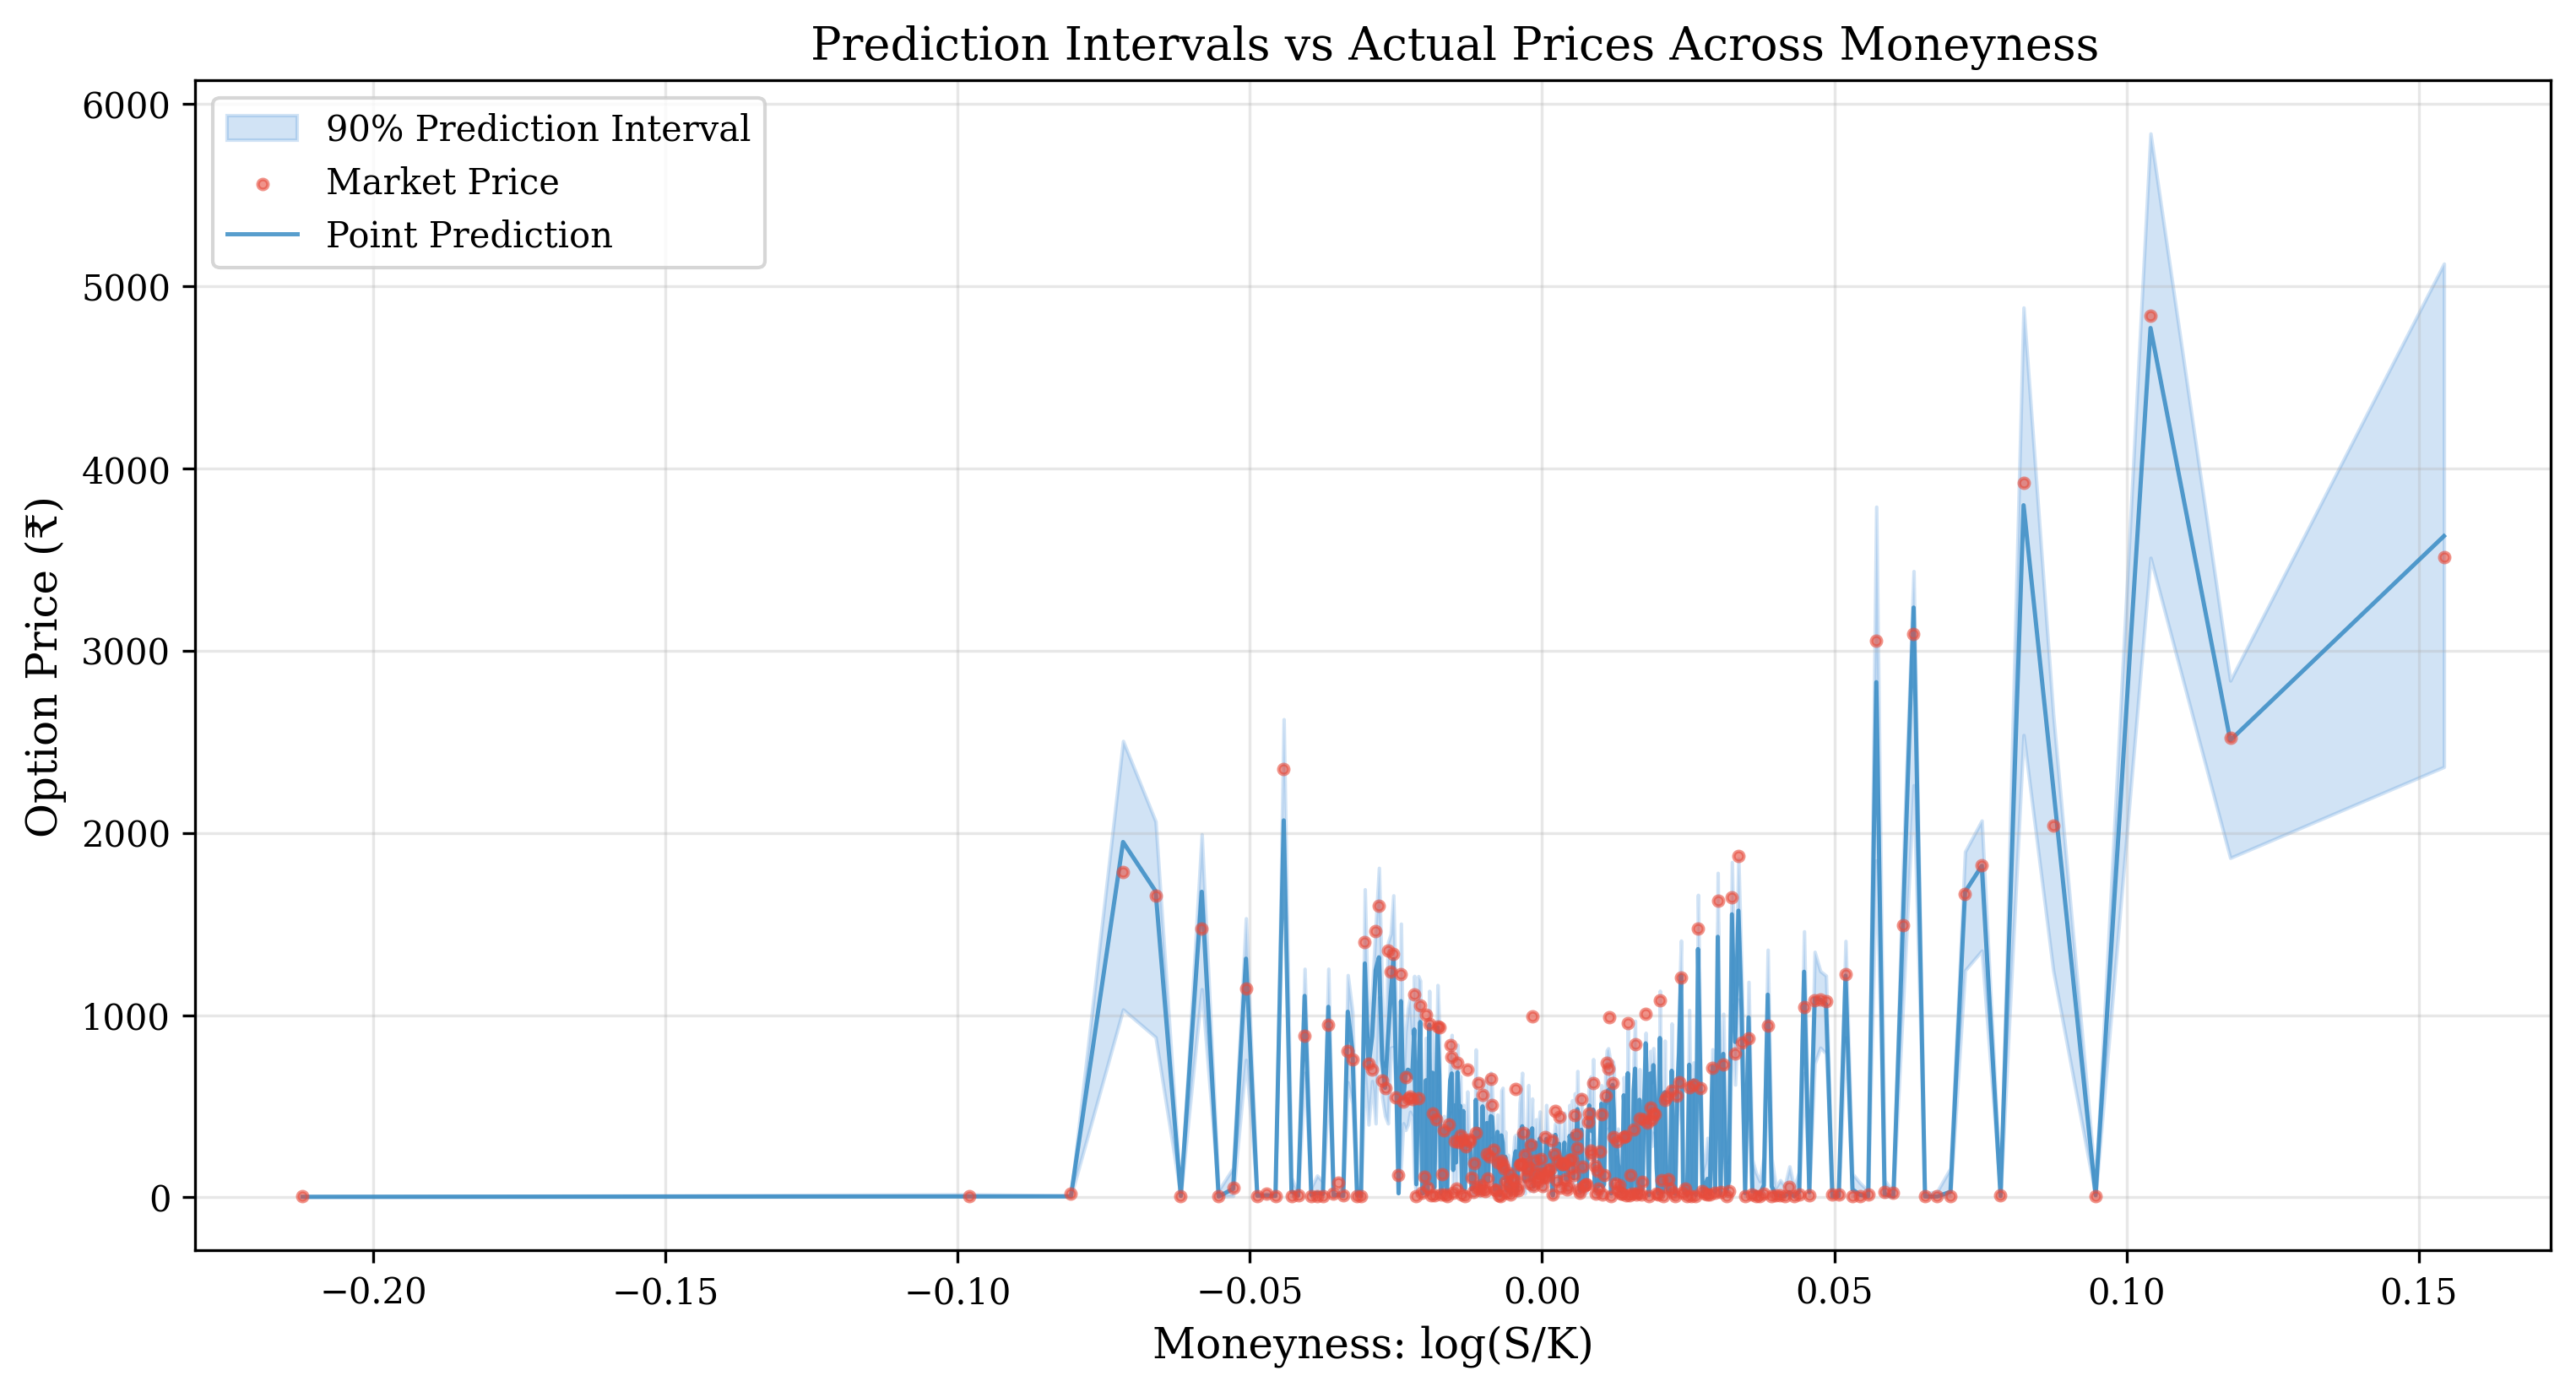
\includegraphics[width=0.9\textwidth]{fig2_intervals.png}
\caption{\rev{Prediction intervals vs. market prices across moneyness. }}
\label{fig:intervals}
\end{figure}

\rev{\textbf{Practical applicability:} The model incorporates meaningful features such as Delta, Vega, option type, rather than opaque statistical patterns, which makes it more suitable for deployment in live trading systems. The conformal calibration layer can be updated without retraining the base model, which can adapt quickly to regime changes. The Normalized Interval Width (average 2.86) can provide traders with an interpretable, scale-free measure of pricing uncertainty.}

A limitation is that the empirical coverage (79.89\%) falls below our 90\% target coverage, suggesting room for improvement. \rev{In the future work, we can incorporate full implied volatility surface learning and integration with transaction costs.}


\section{Conclusion}

\rev{Our research work presents a hybrid option pricing framework that combines BSM as a structural baseline, gradient-boosted quantile regression, which uses BSM Greeks for residual learning, and Asymmetric Conformalized Quantile Regression for distribution-free uncertainty quantification. Evaluated on 3 million intraday NIFTY and BANKNIFTY records, our proposed approach achieves a state-of-the-art point accuracy (MAE 84.06) while providing stable, asymmetric prediction intervals across different moneyness regimes, liquidity conditions, and option types. The framework relies on economically interpretable features such as Delta, Gamma, Vega, and its architecture makes it practical for real-world deployment in trading, hedging, and risk management systems.}


\bibliographystyle{splncs04}
\bibliography{references}

\end{document}
